\documentclass[a4paper,12pt]{article}
\usepackage{CJKutf8}
\usepackage{amsthm}
\usepackage{amsmath}
\usepackage{amssymb}
\usepackage{geometry}
\usepackage{tikz}
\usepackage{tkz-euclide}
\usepackage{tcolorbox}
\usepackage{xcolor}
\usepackage{framed}
\usepackage{listings}
\usepackage[colorlinks,linkcolor=blue,anchorcolor=blue,citecolor=blue]{hyperref}
\tcbuselibrary{skins,listings,fitting,raster}

\geometry{left=3.0cm,right=2.0cm,top=3.0cm,bottom=3.0cm}

\title{\texttt{tkz-euclide} 宏包命令参数展示}
\author{\href{https://logcreative.github.io/LaTeXSparkle/index.html}{\LaTeX\ Sparkle} $\cdot$ \href{https://space.bilibili.com/31271993}{LogCreative}}
\date{}

\begin{document}
\begin{CJK}{UTF8}{gbsn} %需要安装cjk-fonts宏包
\maketitle
%%%%%%%%%%%%%%%%%%%%%%
% tcolorbox 定义
\colorlet{numbar}{red!20!blue!20!white}
\newtcolorbox{commandbox}{
    rightrule=3mm,
    bicolor,
    colback=red!5!white,
    colbacklower=red!10!white,
    colframe=red!75!black,
    sidebyside,
    righthand width=6em,
    halign lower=right,
    before upper=\begin{CJK}{UTF8}{gkai},
    after upper=\end{CJK},
    before lower=\begin{CJK}{UTF8}{gbsn},
    after lower=\end{CJK}
}

\newtcblisting{tikzbox}[4]{
    tikz lower,listing side text,
    coltitle=blue,
    bicolor,colback=blue!5,colbacklower=white,colframe=white,
    righthand width=5cm,
    title={\bfseries \sffamily{#1}\\\rm \color{blue}[\texttt{#2}]\\\color{black}{#3}},
    listing options={
    numbers=left,numberstyle={\ifnum\value{lstnumber}=#4\sffamily\bfseries\scriptsize\color{blue}\else\tiny\color{numbar}\fi},
    %linebackgroundcolor={\ifnum\value{lstnumber}=3\color{green}\fi},
    morekeywords={translation,from,to},columns=fullflexible,basicstyle=\ttfamily\small,keywordstyle=\color{blue}},
    overlay={\begin{tcbclipinterior}\fill[numbar] (frame.south west) rectangle ([xshift=5mm]frame.north west);\end{tcbclipinterior}},
    % before title=\begin{CJK}{UTF8}{kai},
    % after title=\end{CJK},
}

\newtcboxfit{\argbox}[1]{
    colback=white,
    colframe=blue!50,
    title={\bfseries \sffamily{#1}},
    before upper=\begin{CJK}{UTF8}{gbsn},
    after upper=\end{CJK},
    before title=\begin{CJK}{UTF8}{hei},
    after title=\end{CJK},
    %boxsep=0pt,
    top=1mm,bottom=1mm,left=1mm,right=1mm,
}

\newtcboxfit{\auxcombox}[1]{
    colback=white,
    colframe=teal,
    title={\bfseries \texttt{#1}},
    before upper=\begin{CJK}{UTF8}{gbsn},
    after upper=\end{CJK},
    before title=\begin{CJK}{UTF8}{hei},
    after title=\end{CJK},
    %boxsep=0pt,
    top=1mm,bottom=1mm,left=1mm,right=1mm,
}

%%%%%%%%%%%%%%%%%%%%%%

\begin{commandbox}
\verb"\tkzDefPointBy"\textcolor{blue}{[参数]}\textcolor{red}{(参照点)}

\verb"\tkzDefPointsBy"\textcolor{blue}{[参数]}\textcolor{red}{(参照点列表)}\textcolor{teal}{\{定义点列表\}}
\tcblower
变换定义点
\end{commandbox}

\tcbset{fit algorithm=hybrid*}
\begin{tcbraster}[raster columns=3]
    \argbox{translation 平移}{
        \textcolor{blue}{
        \texttt{[translation=from (起始点) to (终止点)]}
        }

        从\textcolor{red}{(参照点)}为始点按照\textcolor{blue}{平移向量}平移得到终点作为定义点。

        \begin{center}
        \begin{tikzpicture}
    \tkzDefPoint(0,0){A} \tkzDefPoint(3,1){B}
    \tkzDefPoint(3,2){C}
    \tkzDefPointBy[translation= from B to A](C)
    \tkzGetPoint{D}
    \tkzDrawPoints[black](A,B,C,D)
    \tkzLabelPoints[color=black](A,B,C)
    \tkzLabelPoints[color=red](D)
    \tkzDrawSegments[orange,<-](A,B D,C)
\end{tikzpicture}
        \end{center}

    }
    \argbox{homothety 位似}{
        \textcolor{blue}{
        \texttt{[homothety=center (位似中心点) ratio (位似比)]}
        }

        从\textcolor{blue}{(位似中心点)}到\textcolor{red}{(参照点)}形成线段(或所在直线上)以\textcolor{blue}{(位似比)}为定比的定比分点。


        \begin{center}
        \begin{tikzpicture}
    \tkzDefPoint(0,0){A} \tkzDefPoint(3,1){B}
    \tkzDefPointBy[homothety=center B ratio 0.5](A)
    \tkzGetPoint{C}
    \tkzDrawPoints(A,B)
    \tkzDrawPoints[red](C)
    \tkzLabelPoints(A,B)
    \tkzLabelPoints[red](C)
    \tkzDrawSegments[->](B,A)
\end{tikzpicture}
        \end{center}
    }
    \argbox{relection 反射}{
        \textcolor{blue}{
        \texttt{[reflection=over (对称轴点1)--(对称轴点2)]}
        }

        对于\textcolor{red}{(参照点)}通过\textcolor{blue}{对称轴}的反射点。

        \begin{center}
        \begin{tikzpicture}
    \tkzDefPoint(0,0){A} \tkzDefPoint(3,1){B}
    \tkzDefPoint(1,2){C}
    \tkzDefPointBy[reflection=over A--B](C)
    \tkzGetPoint{D}
    \tkzDrawPoints[black](A,B,C,D)
    \tkzLabelPoints[color=black](A,B,C)
    \tkzLabelPoints[color=red](D)
    \tkzDrawSegments(A,B)
    \tkzDrawSegment[dashed](C,D)
\end{tikzpicture}
        \end{center}
    }
    \argbox{symmetry 中心对称}{
        \textcolor{blue}{
        \texttt{[symmetry=center (对称中心点)]}
        }

        \textcolor{red}{(参照点)}关于\textcolor{blue}{(对称中心点)}的中心对称点。

        \begin{center}
        \begin{tikzpicture}
    \tkzDefPoint(0,0){O}
    \tkzDefPoint(1,1){A}
    \tkzDefPointBy[symmetry=center O](A)
    \tkzGetPoint{B}
    \tkzDrawPoints[black](O,A)
    \tkzDrawPoints[red](B)
    \tkzLabelPoints(O,A)
    \tkzLabelPoints[red](B)
    \tkzDrawSegment(A,B)
\end{tikzpicture}
        \end{center}
    }
    \argbox{projection 投影}{
        \textcolor{blue}{
        \texttt{[projection=onto 投影轴点1--投影轴点2]}
        }

        \textcolor{red}{(参照点)}在\textcolor{blue}{(投影轴)}上的投影点。

        \begin{center}
        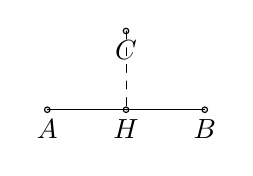
\begin{tikzpicture}
    \tkzDefPoint(0,0){A}
    \tkzDefPoint(2,0){B}
    \tkzDefPoint(1,1){C}
    \tkzDefPointBy[projection=onto A--B](C)
    \tkzGetPoint{H}
    \tkzDrawPoints(A,B,C,H)
    \tkzLabelPoints(A,B,C,H)
    \tkzDrawSegment(A,B)
    \tkzDrawSegment[dashed](C,H)
\end{tikzpicture}
        \end{center}
    }
    \argbox{rotation 旋转}{
        \textcolor{blue}{
            \texttt{[rotation=center (旋转中心点) angle (角度)]}
        }

        \textcolor{red}{(参照点)}绕\textcolor{blue}{(旋转中心点)}旋转\textcolor{blue}{(角度)}得到的点。

        \begin{center}
        \begin{tikzpicture}
    \tkzDefPoint(0,0){O}
    \tkzDefPoint(3,0){A}
    \tkzDefPointBy[rotation=center O angle 30](A)
    \tkzGetPoint{B}
    \tkzDrawPoints(O,A)
    \tkzDrawPoints[red](B)
    \tkzLabelPoints(O,A)
    \tkzLabelPoints[above,red](B)
    \tkzDrawSegments(O,A O,B)
    \tkzMarkAngle[mark=none](A,O,B)
    \tkzLabelAngle[right](A,O,B){$30^{\circ}$}
\end{tikzpicture}
        \end{center}
    }
    \argbox{rotation in rad 弧度旋转}{
        \textcolor{blue}{
            \texttt{[rotation in rad=center (旋转中心点) angle (弧度)]}
        }

        \textcolor{red}{(参照点)}绕\textcolor{blue}{(旋转中心点)}旋转\textcolor{blue}{(弧度)}得到的点。

        \begin{center}
        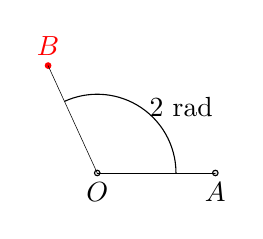
\begin{tikzpicture}
    \tkzDefPoint(0,0){O}
    \tkzDefPoint(1.5,0){A}
    \tkzDefPointBy[rotation in rad=center O angle 2](A)
    \tkzGetPoint{B}
    \tkzDrawPoints(O,A)
    \tkzDrawPoints[red](B)
    \tkzLabelPoints(O,A)
    \tkzLabelPoints[above,red](B)
    \tkzDrawSegments(O,A O,B)
    \tkzMarkAngle[mark=none](A,O,B)
    \tkzLabelAngle[right](A,O,B){2 rad}
\end{tikzpicture}
        \end{center}
    }
    \argbox{inversion 反演}{
        \textcolor{blue}{
            \texttt{[inversion=center (反演中心点) through (反演圆上点)]}
        }

        \textcolor{red}{(参照点)}关于\textcolor{blue}{反演圆}的反演点,满足共线且$OB\times OB'=r^2$。

        \begin{center}
        \begin{tikzpicture}
    \tkzDefPoint(0,0){O}
    \tkzDefPoint(1.5,0){A}
    \tkzDefPoint(0.8,0.3){B}
    \tkzDefPointBy[inversion=center O through A](B)
    \tkzGetPoint{B'}
    \tkzDrawCircle(O,A)
    \tkzDrawPoints(O,B)
    \tkzDrawPoints[red](B')
    \tkzLabelPoints(O,B)
    \tkzLabelPoints[red](B')
    \tkzDrawSegment(B,B')
\end{tikzpicture}
        \end{center}
    }
    \auxcombox{$\backslash$tkzGetPoint 得定义点}{
        ~~~\texttt{$\backslash$tkzDefPointBy}命令后紧跟 \texttt{$\backslash$tkzGetPoint\{结果点\}} 以得到结果。

        ~~~如果使用\texttt{$\backslash$tkzDefPointsBy} 命令,得到的点将直接用\textcolor{teal}{\{定义点列表\}}中的点表示,留空将会使用\textcolor{red}{(参照点)}加撇表示,比如\textcolor{red}{$B$}$\rightarrow$\textcolor{teal}{$B'$}。
    }

\end{tcbraster}

\begin{commandbox}
    \verb"\tkzDefTriangleCenter"\textcolor{blue}{[参数]}\textcolor{red}{(点1,点2,点3)}
    \tcblower
    三角定义点
\end{commandbox}

\begin{tcbraster}[raster columns=3]
    \argbox{ortho 垂心}{
        三角形高的交点。

        \begin{center}
            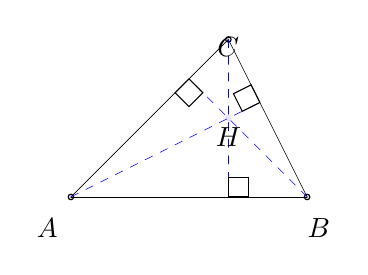
\begin{tikzpicture}
    \tkzDefPoints{0/0/A,3/0/B,2/2/C}
    \tkzDefTriangleCenter[ortho](A,B,C)\tkzGetPoint{H}
    \tkzDrawPoints(A,B,C) \tkzDrawPoints[blue!10](H)
    \tkzDrawSegments(A,B B,C C,A)
    \tkzDefPointBy[projection=onto A--B](C) \tkzGetPoint{H_1}
    \tkzDefPointBy[projection=onto B--C](A) \tkzGetPoint{H_2}
    \tkzDefPointBy[projection=onto C--A](B) \tkzGetPoint{H_3}
    \tkzDrawSegments[dashed,blue](C,H_1 A,H_2 B,H_3)
    \tkzMarkRightAngles(C,H_1,B A,H_2,C B,H_3,A)
    \tkzLabelPoints(H)
    \tkzAutoLabelPoints[center=H](A,B,C)
\end{tikzpicture}
        \end{center}
    }
    \argbox{centroid 重心}{
        三角形中线的交点。

        \begin{center}
            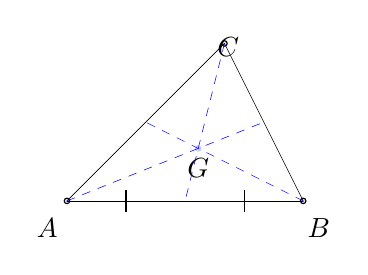
\begin{tikzpicture}
    \tkzDefPoints{0/0/A,3/0/B,2/2/C}
    \tkzDefTriangleCenter[centroid](A,B,C) \tkzGetPoint{G}
    \tkzDrawPoints(A,B,C) \tkzDrawPoints[blue!20](G)
    \tkzDrawSegments(A,B B,C C,A)
    \tkzLabelPoints(G)
    \tkzAutoLabelPoints[center=G](A,B,C)
    \tkzDefMidPoint(A,B) \tkzGetPoint{D}
    \tkzDefMidPoint(B,C) \tkzGetPoint{E}
    \tkzDefMidPoint(C,A) \tkzGetPoint{F}
    \tkzDrawSegments[dashed,blue](C,D A,E B,F)
    \tkzMarkSegments[mark=|](A,D D,B)
\end{tikzpicture}
        \end{center}
    }
    \argbox{circum 外心}{
        三角形外接圆圆心,又是三边中垂线交点。

        \begin{center}
            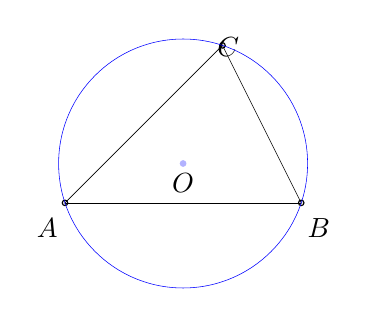
\begin{tikzpicture}
    \tkzDefPoints{0/0/A,3/0/B,2/2/C}
    \tkzDefTriangleCenter[circum](A,B,C) \tkzGetPoint{O}
    \tkzDrawPoints(A,B,C) \tkzDrawPoints[blue!30](O)
    \tkzDrawSegments(A,B B,C C,A)
    \tkzLabelPoints(O)
    \tkzAutoLabelPoints[center=O](A,B,C)
    \tkzDrawCircle[blue](O,A)
\end{tikzpicture}
        \end{center}
    }
    \argbox{in 内心}{
        三角形内切圆圆心,又是三角角分线交点。
        
        \begin{center}
            \begin{tikzpicture}
    \tkzDefPoints{0/0/A,3/0/B,2/2/C}
    \tkzDefTriangleCenter[in](A,B,C) \tkzGetPoint{I}
    \tkzDrawPoints(A,B,C) \tkzDrawPoints[blue!40](I)
    \tkzDrawSegments(A,B B,C C,A)
    \tkzLabelPoints(I)
    \tkzAutoLabelPoints[center=I](A,B,C)
    \tkzDrawCircle[in,blue](A,B,C)
\end{tikzpicture}
        \end{center}
    }
    \argbox{ex 旁心}{
        三角形旁切圆圆心,与\textcolor{red}{点2}的对边相切。

        \begin{center}
            \begin{tikzpicture}[scale=0.6]
    \tkzDefPoints{0/0/B,3/0/A,2/2/C}
    \tkzDefTriangleCenter[ex](A,B,C) \tkzGetPoint{J}
    \tkzDrawPoints(A,B,C) \tkzDrawPoints[blue!50](J)
    \tkzDrawSegments(A,C B,C A,B)
    \tkzDefPointBy[homothety=center B ratio 1.7](C) \tkzGetPoint{D}
    \tkzDefPointBy[homothety=center B ratio 1.7](A) \tkzGetPoint{E}
    \tkzDrawSegments[dashed,blue](C,D A,E)
    \tkzLabelPoints(J)
    \tkzAutoLabelPoints[center=J](A,B,C)
    \tkzDrawCircle[ex,blue](A,B,C)
\end{tikzpicture}
        \end{center}
    }
    \argbox{euler 欧拉圆圆心}{
        三角形垂足三角形外接圆圆心,三角形的三边中点、三个垂心到顶点连线中点也在这个圆上,故该外接圆又称九点圆。

        \begin{center}
            \begin{tikzpicture}
    \tkzDefPoints{0/0/A,3/0/B,2/2/C}
    \tkzDefTriangleCenter[euler](A,B,C) \tkzGetPoint{E}
    \tkzDrawCircle[euler,blue](A,B,C)
    \tkzDefMidPoint(A,B) \tkzGetPoint{M_c}
    \tkzDefMidPoint(A,C) \tkzGetPoint{M_b}
    \tkzDefMidPoint(B,C) \tkzGetPoint{M_a}
    \tkzDrawPoints(A,B,C) \tkzDrawPoints[blue!60](E)
    \tkzDrawPoints[red](M_a,M_b,M_c)
    \tkzDrawSegments(A,B B,C A,C)
    \tkzLabelPoints(E)
    \tkzAutoLabelPoints[center=E](A,B,C)
    \tkzDefPointBy[projection=onto A--B](C) \tkzGetPoint{H_c}
    \tkzDefPointBy[projection=onto B--C](A) \tkzGetPoint{H_a}
    \tkzDefPointBy[projection=onto A--C](B) \tkzGetPoint{H_b}
    \tkzDrawPoints[blue](H_a,H_b,H_c)
    \tkzDrawSegments[blue,dashed](A,H_a B,H_b C,H_c)
    \tkzDefTriangleCenter[ortho](A,B,C) \tkzGetPoint{H}
    \tkzDefMidPoint(A,H) \tkzGetPoint{E_a}
    \tkzDefMidPoint(B,H) \tkzGetPoint{E_b}
    \tkzDefMidPoint(C,H) \tkzGetPoint{E_c}
    \tkzDrawPoints[yellow](E_a,E_b,E_c)
\end{tikzpicture}
        \end{center}
    }
    \argbox{symmedian 类似重心}{
        三角形重心的等角共轭点,也就是中线等角线的交点。

        \begin{center}
            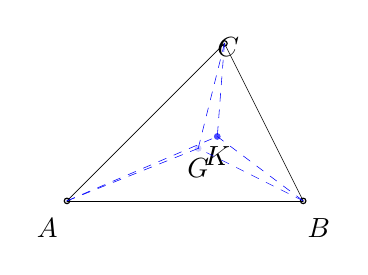
\begin{tikzpicture}
    \tkzDefPoints{0/0/A,3/0/B,2/2/C}
    \tkzDefTriangleCenter[symmedian](A,B,C) \tkzGetPoint{K}
    \tkzDefTriangleCenter[centroid](A,B,C) \tkzGetPoint{G}
    \tkzDrawPoints(A,B,C) \tkzDrawPoints[blue!20](G) \tkzDrawPoints[blue!70](K)
    \tkzDrawSegments(A,B B,C C,A)
    \tkzLabelPoints(G,K)
    \tkzAutoLabelPoints[center=G](A,B,C)
    \tkzDefMidPoint(A,B) \tkzGetPoint{D}
    \tkzDefMidPoint(B,C) \tkzGetPoint{E}
    \tkzDefMidPoint(C,A) \tkzGetPoint{F}
    \tkzDrawSegments[dashed,blue](C,G A,G B,G C,K A,K B,K)
\end{tikzpicture}
        \end{center}
    }
    \argbox{spieker}{
        三角形中点三角形内切圆圆心。

        \begin{center}
            \begin{tikzpicture}
    \tkzDefPoints{0/0/A,3/0/B,2/2/C}
    \tkzDefTriangleCenter[spieker](A,B,C) \tkzGetPoint{S_p}
    \tkzDefMidPoint(A,B) \tkzGetPoint{D}
    \tkzDefMidPoint(B,C) \tkzGetPoint{E}
    \tkzDefMidPoint(C,A) \tkzGetPoint{F}
    \tkzDrawSegments(A,B B,C C,A)
    \tkzDrawSegments[dashed,blue](D,E E,F F,D)
    \tkzDrawCircle[in,blue](D,E,F)
    \tkzAutoLabelPoints[center=S_p](A,B,C,D,E,F)
    \tkzLabelPoints(S_p)
    \tkzDrawPoints(A,B,C,D,E,F) \tkzDrawPoints[blue!80](S_p)
\end{tikzpicture}
        \end{center}
    }
    \argbox{nagel}{
        三角形旁切圆切点与对顶点连线交点。

        \begin{center}
            \begin{tikzpicture}
    \tkzInit[xmin=-1,ymin=-1,xmax=4,ymax=3]
    \tkzClip
    \tkzDefPoints{0/0/A,3/0/B,2/2/C}
    \tkzDefTriangleCenter[nagel](A,B,C) \tkzGetPoint{N_a}
    \tkzDrawCircle[ex,blue](A,B,C)
    \tkzDrawCircle[ex,blue](B,A,C)
    \tkzDrawCircle[ex,blue](A,C,B)
    \tkzDrawSegments[dashed,add=0.5 and 0.5](A,B B,C C,A) 
    \tkzDrawSegments(A,B B,C C,A)
    \tkzDrawPoints(A,B,C) \tkzDrawPoints[blue!90](N_a)
    \tkzDefSpcTriangle[extouch](A,B,C){T_a,T_b,T_c}
    \tkzDrawPoints[blue](T_a,T_b,T_c)
    \tkzDrawSegments[dashed,blue](A,T_a B,T_b C,T_c)
    \tkzLabelPoints(N_a)
    \tkzAutoLabelPoints[center=N_a](A,B,C,T_a,T_b,T_c)
\end{tikzpicture}
        \end{center}
    }
    \argbox{mittenpunkt}{
        三角形旁切圆圆心与中点连线交点。

        \begin{center}
            \begin{tikzpicture}
    \tkzInit[xmin=-1,ymin=-1,xmax=4,ymax=3]
    \tkzClip
    \tkzDefPoints{0/0/A,3/0/B,2/2/C}
    \tkzDefTriangleCenter[mittenpunkt](A,B,C) \tkzGetPoint{M_i}
    \tkzDrawCircle[ex,blue](A,B,C)
    \tkzDrawCircle[ex,blue](B,A,C)
    \tkzDrawCircle[ex,blue](A,C,B)
    \tkzDrawSegments[dashed,add=0.5 and 0.5](A,B B,C C,A) 
    \tkzDrawSegments(A,B B,C C,A)
    \tkzDrawPoints(A,B,C) \tkzDrawPoints[blue](M_i)
    \tkzDefSpcTriangle[centroid](A,B,C){M_a,M_b,M_c}
    % \tkzDrawSegments[dashed,blue](A,T_a B,T_b C,T_c)
    \tkzLabelPoints(M_i)
    \tkzDrawPoints[blue](M_a,M_b,M_c)
    \tkzAutoLabelPoints[center=M_i](A,B,C,M_a,M_b,M_c)
    \tkzDefSpcTriangle[ex](A,B,C){J_a,J_b,J_c}
    %\tkzDrawPoints[red](J_a,J_b,J_c)
    \tkzDrawSegments[red,add=0 and 0.6](J_a,M_a J_b,M_b J_c,M_c)
\end{tikzpicture}
        \end{center}
    }
    \argbox{feuerbach}{
        欧拉圆又称费尔巴哈圆。

        \begin{center}
            \begin{tikzpicture}
    \tkzDefPoints{0/0/A,3/0/B,2/2/C}
    \tkzDefTriangleCenter[euler](A,B,C) \tkzGetPoint{F}
    \tkzDrawCircle[euler,blue](A,B,C)
    \tkzDefMidPoint(A,B) \tkzGetPoint{M_c}
    \tkzDefMidPoint(A,C) \tkzGetPoint{M_b}
    \tkzDefMidPoint(B,C) \tkzGetPoint{M_a}
    \tkzDrawPoints(A,B,C) \tkzDrawPoints[blue!60](F)
    \tkzDrawPoints[red](M_a,M_b,M_c)
    \tkzDrawSegments(A,B B,C A,C)
    \tkzLabelPoints(F)
    \tkzAutoLabelPoints[center=F](A,B,C)
    \tkzDefPointBy[projection=onto A--B](C) \tkzGetPoint{H_c}
    \tkzDefPointBy[projection=onto B--C](A) \tkzGetPoint{H_a}
    \tkzDefPointBy[projection=onto A--C](B) \tkzGetPoint{H_b}
    \tkzDrawPoints[blue](H_a,H_b,H_c)
    \tkzDrawSegments[blue,dashed](A,H_a B,H_b C,H_c)
    \tkzDefTriangleCenter[ortho](A,B,C) \tkzGetPoint{H}
    \tkzDefMidPoint(A,H) \tkzGetPoint{E_a}
    \tkzDefMidPoint(B,H) \tkzGetPoint{E_b}
    \tkzDefMidPoint(C,H) \tkzGetPoint{E_c}
    \tkzDrawPoints[yellow](E_a,E_b,E_c)
\end{tikzpicture}
        \end{center}
    }
    \auxcombox{$\backslash$tkzGetPoint 得定义点}{
        ~~~\texttt{$\backslash$tkzDefTriangleCenter}命令后紧跟 \texttt{$\backslash$tkzGetPoint\{结果点\}} 以得到结果。

        \begin{center}
            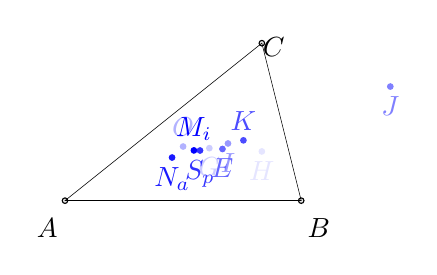
\begin{tikzpicture}
    \tkzDefPoints{0/0/A,3/0/B,2.5/2/C}
    \tkzDrawPoints(A,B,C)
    \tkzDefTriangleCenter[ortho](A,B,C) \tkzGetPoint{H}
    \tkzDefTriangleCenter[centroid](A,B,C) \tkzGetPoint{G}
    \tkzDefTriangleCenter[circum](A,B,C) \tkzGetPoint{O}
    \tkzDefTriangleCenter[in](A,B,C) \tkzGetPoint{I}
    \tkzDefTriangleCenter[ex](B,A,C) \tkzGetPoint{J}
    \tkzDefTriangleCenter[euler](A,B,C) \tkzGetPoint{E}
    \tkzDefTriangleCenter[symmedian](A,B,C) \tkzGetPoint{K}
    \tkzDefTriangleCenter[spieker](A,B,C) \tkzGetPoint{S_p}
    \tkzDefTriangleCenter[nagel](A,B,C) \tkzGetPoint{N_a}
    \tkzDefTriangleCenter[mittenpunkt](A,B,C) \tkzGetPoint{M_i}
    %\tkzDrawPoints(A,B,C,H,G,O,I,J,E,K,S_p,N_a,M_i)
    \tkzAutoLabelPoints[center=O](A,B,C)
    %\tkzLabelPoints[font=\tiny](H,G,O,I,J)
    %\tkzLabelPoints[above,font=\tiny](E,K,S_p,N_a,M_i)
    \tkzDrawSegments(A,B B,C C,A)
    \tkzDrawPoints[blue!10](H) \tkzLabelPoints[blue!10](H)\tkzDrawPoints[blue!20](G) \tkzLabelPoints[blue!20](G)
    \tkzDrawPoints[blue!30](O) \tkzLabelPoints[blue!30,above](O)
    \tkzDrawPoints[blue!40](I) \tkzLabelPoints[blue!40](I)
    \tkzDrawPoints[blue!50](J) \tkzLabelPoints[blue!50](J)
    \tkzDrawPoints[blue!60](E) \tkzLabelPoints[blue!60](E)
    \tkzDrawPoints[blue!70](K) \tkzLabelPoints[blue!70,above](K)
    \tkzDrawPoints[blue!80](S_p) \tkzLabelPoints[blue!80](S_p)
    \tkzDrawPoints[blue!90](N_a) \tkzLabelPoints[blue!90](N_a)
    \tkzDrawPoints[blue](M_i) \tkzLabelPoints[blue,above](M_i)

\end{tikzpicture}
        \end{center}
    }
\end{tcbraster}

\begin{commandbox}
    \verb"\tkzDefLine"\textcolor{blue}{[参数]}\textcolor{red}{(点1,点2\underline{,点3})}
    \tcblower
    定义直线
\end{commandbox}

\begin{tcbraster}[raster columns=3]
    \argbox{mediator 中垂线}{
        \textcolor{red}{(参照线段)}的垂直平分线。

        \begin{center}
            \begin{tikzpicture}
    \tkzDefPoints{0/0/A,2/0/B}
    \tkzDefLine[mediator](A,B)
    \tkzGetPoints{C}{D}
    \tkzDrawPoints(A,B,C,D)
    \tkzDrawSegments(A,B)
    \tkzDrawSegments[red](C,D)
    \tkzDefMidPoint(A,B)
    \tkzGetPoint{E}
    \tkzMarkRightAngles(A,E,C)
    \tkzLabelPoints(A,B,C,D)
\end{tikzpicture}
        \end{center}
    }
    \argbox{perpendicular/orthogonal 垂直}{
        \textcolor{blue}{
            \texttt{[perpendicular=through (经过点)]}
        }

        % \textcolor{blue}{
        %     \texttt{[orthogonal=through (经过点)]}
        % }

        过\textcolor{blue}{(经过点)}关于\textcolor{red}{(参照线段)}的垂直线。

        \begin{center}
            \begin{tikzpicture}
    \tkzDefPoints{0/0/A,2/0/B}
    \tkzDefLine[perpendicular=through A](A,B)
    \tkzGetPoint{C}
    \tkzDrawPoints(A,B,C)
    \tkzDrawSegments(A,B)
    \tkzDrawSegments[red](A,C)
    \tkzLabelPoints(A,B,C)
    \tkzMarkRightAngles(C,A,B)
\end{tikzpicture}
        \end{center}
    }
    \argbox{parallel 平行}{
        \textcolor{blue}{
            \texttt{[parallel=through (经过点)]}
        }
        
        过\textcolor{blue}{(经过点)}关于\textcolor{red}{(参照线段)}的平行线。

        \begin{center}
            \begin{tikzpicture}
    \tkzDefPoints{0/0/A,1.5/0/B,1/1/C}
    \tkzDefLine[parallel=through C](A,B)
    \tkzGetPoint{D}
    \tkzDrawSegments(A,B)
    \tkzDrawSegments[red](C,D)
    \tkzDrawPoints(A,B,C)
    \tkzDrawPoints[red](D)
    \tkzLabelPoints(A,B,C,D)
\end{tikzpicture}
        \end{center}
    }
    \argbox{bisector 角分线}{
        作以\textcolor{red}{(点2)}为角点的内角平分线。注意角度要以逆时针方向标记。

        \begin{center}
            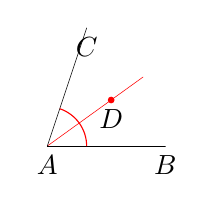
\begin{tikzpicture}
    \tkzDefPoints{0/0/A,1.5/0/B,0.5/1.5/C}
    \tkzDefLine[bisector,normed](B,A,C)
    \tkzGetPoint{D}
    \tkzDrawLines[red,add=0 and 0.5](A,D)
    \tkzDrawPoints[red](D)
    % \tkzDrawPoints(A,B,C)
    \tkzLabelPoints(A,B,C,D)
    \tkzDrawSegments(A,B A,C)
    \tkzMarkAngles[mark=none,red,size=0.5cm](B,A,D D,A,C)
\end{tikzpicture}
        \end{center}
    }
    \argbox{bisector out 补角分线}{
        作以\textcolor{red}{(点2)}为角点的补角平分线。

        \begin{center}
            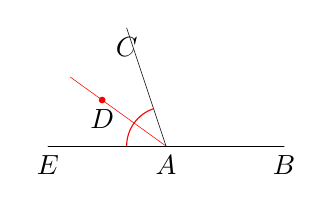
\begin{tikzpicture}
    \tkzDefPoints{0/0/A,1.5/0/B,-0.5/1.5/C,-1.5/0/E}
    \tkzDefLine[bisector out,normed](B,A,C)
    \tkzGetPoint{D}
    \tkzDrawLines[red,add=0 and 0.5](A,D)
    \tkzDrawPoints[red](D)
    % \tkzDrawPoints(A,B,C,E)
    \tkzLabelPoints(A,B,C,D,E)
    \tkzDrawSegments(A,B A,C A,E)
    \tkzMarkAngles[mark=none,red,size=0.5cm](C,A,D D,A,E)
\end{tikzpicture}
        \end{center}
    }
    \auxcombox{$\backslash$tkzGetPoints 得端点}{
        第一个命令有两个结果,通过\textbackslash\texttt{tkzGetPoints}\{线点1\}\{线点2\} 得到。
        
        后面四个命令只有一个结果,通过\textbackslash\texttt{tkzGetPoint}(线点) 得到。
    }
\end{tcbraster}

\begin{commandbox}
    \verb"\tkzInter__"\textcolor{blue}{[参数]}\textcolor{red}{(点1,点2)(点3,点4)}
    \tcblower
    交点
\end{commandbox}

\begin{tcbraster}[raster columns=3,height=10cm]
    \auxcombox{$\backslash$tkzInterLL 直线交点}{
        两条相交直线的交点。

        \begin{center}
            \begin{tikzpicture}
    \tkzDefPoints{-1/0/A,1/0/B,0.5/2.5/C,-0.5/-1.5/D}
    \tkzInterLL(A,B)(C,D)
    \tkzGetPoint{E}
    \tkzDrawSegments(A,B C,D)
    \tkzDrawPoints(A,B,C,D)
    \tkzDrawPoints[red](E)
    \tkzLabelPoints(A,B,C,D,E)
\end{tikzpicture}
        \end{center}

        交点通过 \textbackslash\texttt{tkzGetPoint} (交点) 得到。

    }
    \auxcombox{$\backslash$tkzInterLC 线圆交点}{
        直线与圆的交点。

        \texttt{
            \textbackslash tkzInterLC\textcolor{red}{(直线点1,直线点2)(圆心,圆上点)}
        }

        \begin{center}
            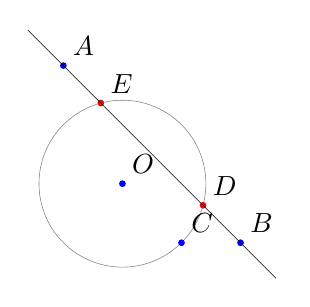
\begin{tikzpicture}[scale=.75]
    \tkzInit[xmax=5,ymax=4]
    \tkzDefPoint(1,1){O}
    \tkzDefPoint(0,3){A}
    \tkzDefPoint(3,0){B}
    \tkzDefPoint(2,0){C}
    \tkzInterLC(A,B)(O,C) \tkzGetPoints{D}{E}
    \tkzDrawCircle(O,C)
    \tkzDrawPoints[color=blue](O,A,B,C)
    \tkzDrawPoints[color=red](D,E)
    \tkzDrawLine(A,B)
    \tkzLabelPoints[above right](O,A,B,C,D,E)
\end{tikzpicture}
        \end{center}

        \texttt{
            \textbackslash tkzInterLC\textcolor{blue}{[R]}\textcolor{red}{(直线点1,直线点2)(圆心,半径)}
        }

        % \begin{center}
        %     \begin{tikzpicture}
    \tkzDefPoints{0/0/O,1.2/0.5/A,-1.25/0.75/B}
    \tkzInterLC[R](A,B)(O,1 cm)
    \tkzGetPoints{C}{D}
    \tkzDrawCircle[R](O,1 cm)
    \tkzDrawSegments[add=0.25 and 0.25](A,B)
    \tkzDrawPoints(O,A,B)
    \tkzDrawPoints[red](C,D)
    \tkzLabelPoints(O,A,B)
    \tkzLabelPoints[above](C,D)  
\end{tikzpicture}
        % \end{center}

        两个交点通过 \textbackslash\texttt{tkzGetPoints} \{交点1\}\{交点2\} 得到。
    }
    \auxcombox{$\backslash$tkzInterCC 圆圆交点}{
        两相交圆交点。

        \texttt{$\backslash$tkzInterCC\textcolor{red}{(圆心1,圆上点1)(圆心2,圆上点2)}}

        \begin{center}
            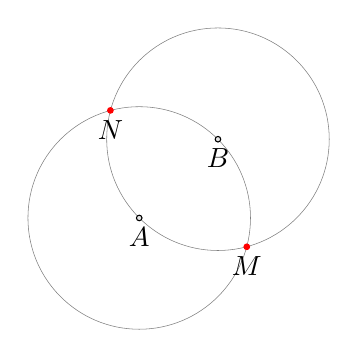
\begin{tikzpicture}[scale=.5]
    \tkzDefPoint(0,0){A}
    \tkzDefPoint(2,2){B}
    \tkzDrawCircle(B,A)
    \tkzDrawCircle(A,B)
    \tkzInterCC(B,A)(A,B)\tkzGetPoints{M}{N}
    \tkzDrawPoints(A,B)
    \tkzDrawPoints[red](M,N)
    \tkzLabelPoints(A,B,M,N)
\end{tikzpicture}
        \end{center}

        两个交点通过 \textbackslash\texttt{tkzGetPoints} \{交点1\}\{交点2\} 得到。
    }
\end{tcbraster}

\begin{commandbox}
    \verb"\tkzDefTriangle"\textcolor{blue}{[参数]}\textcolor{red}{(点1,点2)}
    \tcblower
    定义三角形
\end{commandbox}

\begin{tcbraster}[raster columns=3]
    \argbox{two angles 两角}{
        \textcolor{blue}{
            \texttt{[two angles=(底角1) and (底角2)]}
        }

        指定\textcolor{blue}{两个底角}确定第三点位置。

        \begin{center}
            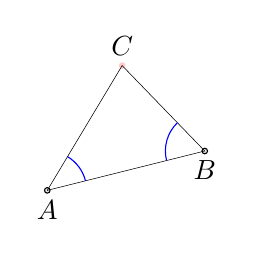
\begin{tikzpicture}
	\tkzDefPoints{0/0/A,2/0.5/B}
	\tkzDefTriangle[two angles=45 and 60](A,B)
	\tkzGetPoint{C}
	\tkzDrawPoints(A,B)
	\tkzDrawPoints[red!20](C)
	\tkzDrawSegments(A,B B,C C,A)
	\tkzLabelPoints(A,B)
	\tkzLabelPoints[above](C)
	\tkzMarkAngles[blue,size=0.5cm,mark=none](B,A,C C,B,A)
\end{tikzpicture}
        \end{center}
    }
    \argbox{equilateral 等边}{
        以\textcolor{red}{指定边}作等边三角形。

        \begin{center}
            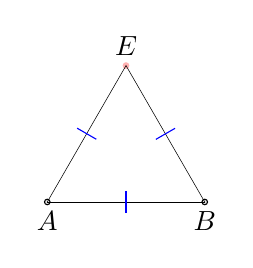
\begin{tikzpicture}
	\tkzDefPoints{0/0/A,2/0/B}
	\tkzDefTriangle[equilateral](A,B)
	\tkzGetPoint{E}
	\tkzDrawPoints(A,B)
	\tkzDrawPoints[red!30](E)
	\tkzDrawSegments(A,B B,E E,A)
	\tkzLabelPoints(A,B)
    \tkzLabelPoints[above](E)
    \tkzMarkSegments[blue](A,B B,E E,A)
\end{tikzpicture}
        \end{center}
    }
    \argbox{pythagore 毕达哥拉斯}{
        等比例于 3-4-5 三角形。

        \begin{center}
            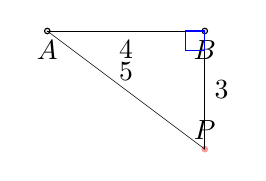
\begin{tikzpicture}
	\tkzDefPoints{0/0/A,2/0/B}
	\tkzDefTriangle[pythagore](A,B)
	\tkzGetPoint{P}
	\tkzDrawPoints(A,B)
	\tkzDrawPoints[red!40](P)
	\tkzDrawSegments(A,B B,P P,A)
	\tkzLabelPoints(A,B)
	\tkzLabelPoints[above](P)
	\tkzMarkRightAngle[blue](P,B,A)
	\tkzLabelSegment[below](A,B){4}
	\tkzLabelSegment[right](B,P){3}
	\tkzLabelSegment[above](P,A){5}
\end{tikzpicture}
        \end{center}
    }
    \argbox{school 三角板}{
        有一内角为 $30^\circ$ 的直角三角形。

        \begin{center}
            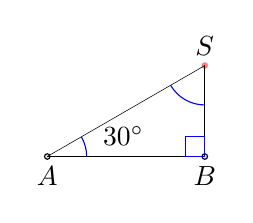
\begin{tikzpicture}
	\tkzDefPoints{0/0/A,2/0/B}
	\tkzDefTriangle[school](A,B)
	\tkzGetPoint{S}
	\tkzDrawPoints(A,B)
	\tkzDrawPoints[red!50](S)
	\tkzDrawSegments(A,B B,S S,A)
	\tkzLabelPoints(A,B)
	\tkzLabelPoints[above](S)
	\tkzMarkRightAngle[blue](S,B,A)
	\tkzMarkAngles[size=0.5cm,mark=none,blue](B,A,S A,S,B)
	\tkzLabelAngle(B,A,S){$30^\circ$}
\end{tikzpicture}
        \end{center}
    }
    \argbox{gold/euclide 欧几里得}{
        顶角为 $36^\circ$ 的等腰三角形。

        区别在于\textcolor{blue}{\texttt{gold}}以\textcolor{red}{(点1)}为顶点,\textcolor{blue}{\texttt{euclide}}以\textcolor{red}{指定边}为底边。

        \begin{center}
            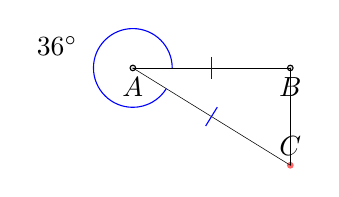
\begin{tikzpicture}
	\tkzDefPoints{0/0/A,2/0/B}
	\tkzDefTriangle[gold](A,B)
	\tkzGetPoint{C}
	\tkzDrawPoints(A,B)
	\tkzDrawPoints[red!60](C)
	\tkzDrawSegments(A,B B,C C,A)
	\tkzLabelPoints(A,B)
	\tkzLabelPoints[above](C)
	\tkzMarkAngles[size=0.5cm,mark=none,blue](B,A,C)
	\tkzLabelAngle(B,A,C){$36^\circ$}
	\tkzMarkSegments[blue](A,B A,C)
\end{tikzpicture}
        \end{center}
    }
    \argbox{golden 黄金三角形}{
        长直角边与短直角边的边长比为$\Phi=1.618$的直角三角形,由黄金矩形的概念衍生而来。

        \begin{center}
            \begin{tikzpicture}
	\tkzDefPoints{0/0/A,2/0/B}
	\tkzDefTriangle[golden](A,B)
	\tkzGetPoint{G}
	\tkzDrawPoints(A,B)
	\tkzDrawPoints[red!70](G)
	\tkzDrawSegments(A,B B,G G,A)
	\tkzLabelPoints(A,B)
	\tkzLabelPoints[above](G)
	\tkzDrawLine[bisector,dashed](B,G,A)
\end{tikzpicture}
        \end{center}
    }
    \argbox{cheops 齐奥普斯}{
        以\textcolor{red}{指定边}为底边、腰长与底边长比例为$\frac{\Phi}{2}$的等腰三角形。

        \begin{center}
            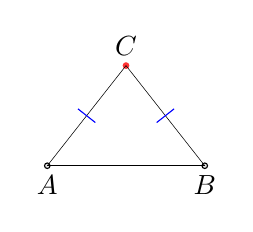
\begin{tikzpicture}
	\tkzDefPoints{0/0/A,2/0/B}
	\tkzDefTriangle[cheops](A,B)
	\tkzGetPoint{C}
	\tkzDrawPoints(A,B)
	\tkzDrawPoints[red!80](C)
	\tkzDrawSegments(A,B B,C C,A)
	\tkzLabelPoints(A,B)
	\tkzLabelPoints[above](C)
	\tkzMarkSegments[blue](A,C B,C)
\end{tikzpicture}
        \end{center}
    }
    \auxcombox{$\backslash$tkzGetPoint 第三点}{
        \texttt{$\backslash$tkzDefTriangle}命令后紧跟 \texttt{$\backslash$tkzGetPoint\{结果点\}} 以得到三角形的第三点。

        \begin{center}
            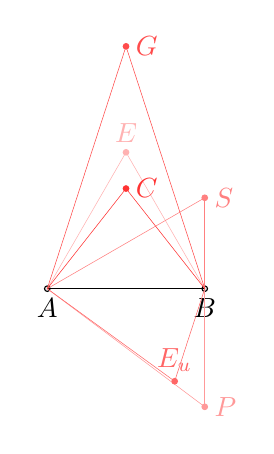
\begin{tikzpicture}
	\tkzDefPoints{0/0/A,2/0/B}
	\tkzDrawPoints(A,B)
	\tkzDrawSegment(A,B)
	\tkzLabelPoints(A,B)
	\tkzDefTriangle[equilateral](A,B)
	\tkzGetPoint{E}
	\tkzDrawPoints[red!30](E)
	\tkzDrawSegments[red!30](A,E B,E)
	\tkzLabelPoints[red!30,above](E)
	\tkzDefTriangle[pythagore](A,B)
	\tkzGetPoint{P}
	\tkzDrawPoints[red!40](P)
	\tkzDrawSegments[red!40](A,P B,P)
	\tkzLabelPoints[red!40,right](P)
	\tkzDefTriangle[school](A,B)
	\tkzGetPoint{S}
	\tkzDrawPoints[red!50](S)
	\tkzDrawSegments[red!50](A,S B,S)
	\tkzLabelPoints[red!50,right](S)
	\tkzDefTriangle[euclide](A,B)
	\tkzGetPoint{E_u}
	\tkzDrawPoints[red!60](E_u)
	\tkzDrawSegments[red!60](A,E_u B,E_u)
	\tkzLabelPoints[red!60,above](E_u)
	\tkzDefTriangle[golden](A,B)
	\tkzGetPoint{G}
	\tkzDrawPoints[red!70](G)
	\tkzDrawSegments[red!70](A,G B,G)
	\tkzLabelPoints[red!70,right](G)
		\tkzDefTriangle[cheops](A,B)
	\tkzGetPoint{C}
	\tkzDrawPoints[red!80](C)
	\tkzDrawSegments[red!80](A,C B,C)
	\tkzLabelPoints[red!80,right](C)
\end{tikzpicture}
        \end{center}
    }
    \auxcombox{tkzPointResult 得变量}{
        如果第三点只用一次,可以使用\texttt{\textbackslash tkzPointResult}临时变量。
    }
\end{tcbraster}

\begin{commandbox}
    \verb"\tkzDefTangent"\textcolor{blue}{[参数]}\textcolor{red}{(点1,点2)}
    \tcblower
    定义切线
\end{commandbox}

\begin{tcbraster}[raster columns=3,height=4.5cm]
    \argbox{at}{

    }
    \argbox{from}{

    }
    \argbox{from with R}{

    }
\end{tcbraster}

\begin{commandbox}
    \verb"\tkzDefCircle"\textcolor{blue}{[参数]}\textcolor{red}{(点1,点2\underline{,点3})}
    \tcblower
    定义圆
\end{commandbox}

\begin{tcbraster}[raster columns=3]
    \argbox{through 半径}{
        以\textcolor{red}{(点1)}为圆心,\textcolor{red}{(点2)}为圆上点定义圆。

        \begin{center}
            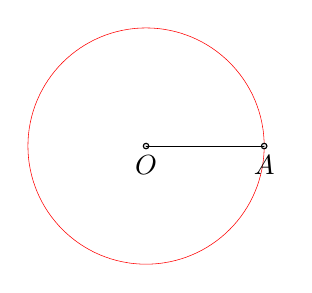
\begin{tikzpicture}
    \tkzDefPoints{0/0/O,1.5/0/A}
    % \tkzDefCircle(O,A)
    \tkzDrawCircle[red](O,A)
    \tkzDrawPoints(O,A)
    \tkzLabelPoints(O,A)
    \tkzDrawSegments(O,A)
\end{tikzpicture}
        \end{center}
    }
    \argbox{diameter 直径}{
        以\textcolor{red}{(参照点)}定义的\textcolor{red}{直径}定义圆。

        \begin{center}
            \begin{tikzpicture}
    \tkzDefPoints{-1.5/0/B,1.5/0/A}
    \tkzDefCircle[diameter](B,A)
    \tkzGetPoint{O}
    \tkzDrawCircle[red,diameter](B,A)
    \tkzDrawPoints(O,B,A)
    \tkzLabelPoints(O,B,A)
    \tkzDrawSegments(B,A)
\end{tikzpicture}
        \end{center}
    }
    \argbox{circum 外接圆}{
        \textcolor{red}{(参照点)}所定义的\textcolor{red}{(三角形)}的外接圆。

        \begin{center}
            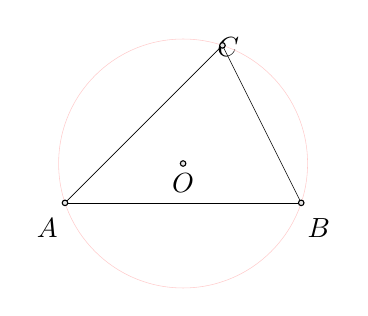
\begin{tikzpicture}
    \tkzDefPoints{0/0/A,3/0/B,2/2/C}
    % \tkzDefTriangleCenter[circum](A,B,C) \tkzGetPoint{O}
    % \tkzDrawPoints(A,B,C) \tkzDrawPoints[blue!30](O)
    \tkzDrawSegments(A,B B,C C,A)
    \tkzDefCircle[circum](A,B,C)
    \tkzGetPoint{O}
    \tkzLabelPoints(O)
    \tkzAutoLabelPoints[center=O](A,B,C)
    \tkzDrawCircle[red!20](O,A)
    \tkzDrawPoints(O,A,B,C)
\end{tikzpicture}
        \end{center}
    }
    \argbox{in 内切圆}{
        \textcolor{red}{(参照点)}所定义的\textcolor{red}{(三角形)}的内切圆。

        \begin{center}
            \begin{tikzpicture}
    \tkzDefPoints{0/0/A,3/0/B,2/2/C}
    \tkzDefCircle[in](A,B,C)
    \tkzGetPoint{I} \tkzGetLength{ls}
    \tkzDrawCircle[R,red](I, \ls pt)
    \tkzDrawPoints(I,A,B,C)
    \tkzLabelPoints(I)
    \tkzAutoLabelPoints[center=I](A,B,C)
    \tkzDrawSegments(A,B B,C C,A)
\end{tikzpicture}
        \end{center}
    }
    \argbox{ex 旁切圆}{
        \textcolor{red}{(参照点)}所定义的\textcolor{red}{(三角形)}与\textcolor{red}{(点2)}相对的旁切圆。

        \begin{center}
            \begin{tikzpicture}[scale=0.6]
    \tkzDefPoints{0/0/B,3/0/A,2/2/C}
    \tkzDefCircle[ex](A,B,C) \tkzGetPoint{J} \tkzGetLength{ls}
    \tkzDrawPoints(A,B,C) \tkzDrawPoints(J)
    \tkzDrawSegments(A,C B,C A,B)
    \tkzDefPointBy[homothety=center B ratio 1.7](C) \tkzGetPoint{D}
    \tkzDefPointBy[homothety=center B ratio 1.7](A) \tkzGetPoint{E}
    \tkzDrawSegments[dashed,blue](C,D A,E)
    \tkzLabelPoints(J)
    \tkzAutoLabelPoints[center=J](A,B,C)
    \tkzDrawCircle[R,red](J, \ls pt)
\end{tikzpicture}
        \end{center}
    }
    \argbox{euler 欧拉圆}{
        \textcolor{red}{(参照点)}所定义\textcolor{red}{(三角形)}的欧拉圆。

        \begin{center}
            \begin{tikzpicture}
    \tkzDefPoints{0/0/A,3/0/B,2/2/C}
    \tkzDefCircle[euler](A,B,C)
    \tkzGetPoint{E} \tkzGetLength{els}
    \tkzDrawCircle[R,red](E,\els pt)
    \tkzDrawSegments(A,B B,C C,A)
    \tkzDrawPoints(A,B,C,E)
    \tkzLabelPoints(E)
    \tkzAutoLabelPoints[center=E](A,B,C)
\end{tikzpicture}
        \end{center}
    }
    \argbox{apollonius 阿波罗尼斯圆,K=比例}{
        到\textcolor{red}{(点1)}的距离与到\textcolor{red}{(点2)}的距离比例为$K$的动点轨迹。

        \begin{center}
            \begin{tikzpicture}[scale=0.8]
    \tkzDefPoints{0/0/A,2/0/B}
    \tkzDefCircle[apollonius,K=2](A,B)
    \tkzGetPoint{O} \tkzGetLength{ar}
    \tkzDrawCircle[R,red](O,\ar pt)
    \tkzDefRandPointOn[circle=center O radius \ar pt]
    \tkzGetPoint{P}
    \tkzDrawPoints(A,B,O,P)
    \tkzDrawSegments(A,B P,A P,B)
    \tkzLabelPoints(O,A,B,P)
\end{tikzpicture}
        \end{center}
    }
    % \argbox{spieker}{
    %     三角形中点三角形内切圆。
    % % 该命令有 bug。
    %     \begin{center}
    %         \input{pic/Cspieker.tex}
    %     \end{center}
    % }
    \argbox{orthogonal 正交圆}{
        正交两圆在交点处切线相互垂直。

        \textcolor{blue}{
            \texttt{[orthogonal from=(圆心)]}
        }

        其后需要紧跟
        
        $\backslash$\texttt{tkzGetPoints}\{(圆上点)\} \{(圆上点)\} 得到结果。 %tcolorbox 中的内容不允许使用\verb

        \textcolor{blue}{
            \texttt{[orthogonal through=(圆上点1) and (圆上点2)]}
        }

    }
    \argbox{orthogonal from}{
        以指定的 \textcolor{blue}{(圆心)} 作以 \textcolor{red}{(点1)} 为圆心、 \textcolor{red}{(点2)} 为圆上点的正交圆。

        \begin{center}
            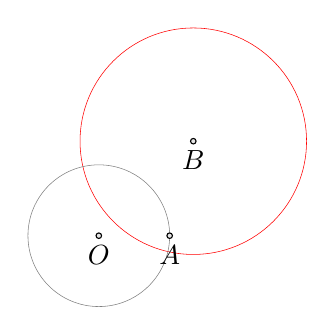
\begin{tikzpicture}[scale=0.6]
    \tkzDefPoints{0/0/O,1.5/0/A,2/2/B}
    \tkzDefCircle[orthogonal from=B](O,A) 
    \tkzGetPoints{z1}{z2}
    \tkzDrawCircle[red](B,z1)
    \tkzDrawCircle(O,A)
    \tkzDrawPoints(O,A,B)
    \tkzLabelPoints(O,A,B)
    \tkzInterCC(O,A)(B,z1)
    % \tkzGetPoints{C}{D}
    % \tkzDrawSegments[dashed,blue](O,C O,D B,C B,D)
    % \tkzDrawPoints(C,D)
    % \tkzMarkRightAngles(B,C,O B,D,O)
\end{tikzpicture}
        \end{center}
    }
    \argbox{orthogonal through}{
        以指定的 \textcolor{blue}{(圆上点1)} 、 \textcolor{blue}{(圆上点2)} 作以 \textcolor{red}{(点1)} 为圆心、 \textcolor{red}{(点2)} 为圆上点的正交圆。
        
        \begin{center}
            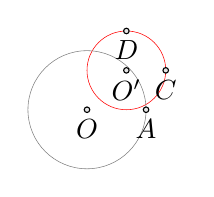
\begin{tikzpicture}[scale=0.5]
    \tkzDefPoints{0/0/O,1.5/0/A,2/1/C,1/2/D}
    \tkzDefCircle[orthogonal through=C and D](O,A) 
    \tkzGetPoint{O'}
    \tkzDrawCircle[red](O',C)
    \tkzDrawCircle(O,A)
    \tkzDrawPoints(O,A,C,D,O')
    \tkzLabelPoints(O,A,C,D,O')
    \tkzInterCC(O,A)(O',C)
    \tkzGetPoints{E}{F}
    % \tkzDrawPoints(E,F)
    % \tkzDrawSegments[dashed,blue](O,E E,O' O,F F,O')
    % \tkzMarkRightAngles(O,E,O' O,F,O')
    % \tkzDefTangent[at=O](E)
    % \tkzGetPoint{h}
    % \tkzDefTangent[at=O'](E)
    % \tkzGetPoint{h'}
    % \tkzDrawSegments[blue,dashed](E,h E,h')
\end{tikzpicture}
        \end{center}

    }
    \auxcombox{$\backslash$tkzGetPoint 得圆心}{
        在命令后紧跟
        
        $\backslash$\texttt{tkzGetPoint}\{\{圆心\}\} 一般可以得到圆心点。
    }
    \auxcombox{$\backslash$tkzGetLength 得半径}{
        在命令后紧跟
        
        $\backslash$\texttt{tkzGetLength}\{(长度变量)\} 可以得到半径,而后使用 $\backslash$\texttt{tkzDrawCircle((圆心),$\backslash$(长度变量) pt)} 画出该圆。
    }

\end{tcbraster}

\end{CJK}
\end{document} 